\documentclass[12pt]{article}
\usepackage[top=1in, bottom=1in, left=.75in, right=.75in]{geometry}
\usepackage{amsmath}
\usepackage{fancyhdr}
\usepackage{graphicx}
\usepackage{txfonts}
\usepackage{multicol,coordsys}
\usepackage[scaled=0.86]{helvet}
\renewcommand{\emph}[1]{\textsf{\textbf{#1}}}
\usepackage{anyfontsize}
% \usepackage{times}
% \usepackage[lf]{MinionPro}
\usepackage{tikz,pgfplots,mathrsfs}
%\def\degC{{}^\circ{\rm C}}
\def\ra{\rightarrow}
\usetikzlibrary{calc, backgrounds}
\pgfplotsset{compat = newest}
\newcommand{\blank}[1]{\rule{#1}{0.75pt}}

\pgfplotsset{my style/.append style={axis x line=middle, axis y line=
middle, xlabel={$x$}, ylabel={$y$},axis equal}}

%yticklabels={,,} , xticklabels={,,}

% \setmainfont{Times}
% \def\sansfont{Lucida Grande Bold}
\parindent 0pt
\parskip 4pt
\pagestyle{fancy}
\fancyfoot[C]{\emph{\thepage}}
\fancyhead[L]{\ifnum \value{page} > 1\relax\emph{Math 251: Final Exam}\fi}
\fancyhead[R]{\ifnum \value{page} > 1\relax\emph{Spring 2023}\fi}
\headheight 15pt
\renewcommand{\headrulewidth}{0pt}
\renewcommand{\footrulewidth}{0pt}
\let\ds\displaystyle
\def\continued{{\emph {Continued....}}}
\def\continuing{{\emph {Problem \arabic{probcount} continued....}}\par\vskip 4pt}


\newcounter{probcount}
\newcounter{subprobcount}
\newcommand{\thesubproblem}{\emph{\alph{subprobcount}.}}
\def\problem#1{\setcounter{subprobcount}{0}%
\addtocounter{probcount}{1}{\emph{\arabic{probcount}.\hskip 1em(#1)}}\par}
\def\subproblem#1{\par\hangindent=1em\hangafter=0{%
\addtocounter{subprobcount}{1}\thesubproblem\emph{#1}\hskip 1em}}
\def\probskip{\vskip 10pt}
\def\medprobskip{\vskip 2in}
\def\subprobskip{\vskip 45pt}
\def\bigprobskip{\vskip 4in}

\begin{document}
{\emph{\fontsize{26}{28}\selectfont Math F251\hfill
{\fontsize{32}{36}\selectfont Final Exam}
\hfill Spring 2023}}
\vskip 2cm
\strut\vtop{\halign{\emph#\hskip 0.5em\hfil&#\hbox to 2in{\hrulefill}\cr
\emph{\fontsize{18}{22}\selectfont Name:}&\cr
\noalign{\vskip 10pt}}}
%%\emph{\fontsize{18}{22}\selectfont Student Id:}&\cr
%%\noalign{\vskip 10pt}
%%\emph{\fontsize{18}{22}\selectfont Calculator Model:}&\cr
%}}
%\hfill
%\vtop{\halign{\emph{\fontsize{18}{22}\selectfont #}\hfil& \emph{\fontsize{18}{22}\selectfont\hskip 0.5ex $\square$ #}\hfil\cr
%Section: & 001 (Jill Faudree)\cr
%\noalign{\vskip 4pt}
%         & 002 (James Gossell)\cr
%\noalign{\vskip 4pt}
%         & 005 (James Gossell)\cr}}

\vfill
{\fontsize{18}{22}\selectfont\emph{Rules:}}

You have 2 hours to complete the final exam.  

Partial credit will be awarded, but you must show your work.

You may have a single handwritten $3 \times 5$ notecard.

Calculators are not allowed. 


Place a box around your  \fbox{FINAL ANSWER} to each question where appropriate.

%If you need extra space, you can use the back sides of the pages.
%Please make it obvious  when you have done so.

Turn off anything that might go beep during the exam.

Good luck!
\vfill
\def\emptybox{\hbox to 2em{\vrule height 16pt depth 8pt width 0pt\hfil}}
\def\tline{\noalign{\hrule}}
\centerline{\vbox{\offinterlineskip
{
\bf\sf\fontsize{18pt}{22pt}\selectfont
\hrule
\halign{
\vrule#&\strut\quad\hfil#\hfil\quad&\vrule#&\quad\hfil#\hfil\quad
&\vrule#&\quad\hfil#\hfil\quad&\vrule#\cr
height 3pt&\omit&&\omit&&\omit&\cr
&Problem&&Possible&&Score&\cr\tline
height 3pt&\omit&&\omit&&\omit&\cr
&1&&8&&\emptybox&\cr\tline
&2&&8&&\emptybox&\cr\tline
&3&&8&&\emptybox&\cr\tline
&4&&10&&\emptybox&\cr\tline
&5&&12&&\emptybox&\cr\tline
&6&&10&&\emptybox&\cr\tline
&7&&12&&\emptybox&\cr\tline
&8&&12&&\emptybox&\cr\tline
&9&&12&&\emptybox&\cr\tline
&10&&8&&\emptybox&\cr\tline
&Extra Credit&&5&&\emptybox&\cr\tline
&Total&&100&&\emptybox&\cr
}\hrule}}}

\newpage
\begin{enumerate}
%%% straight limits
%%DRAFTED
\item (8 points) Evaluate the limits. An answer without clear, mathematically precise work, will not earn full credit. Any use of L'H\^{o}pital's Rule should be indicated using an \textbf{H} over the equal sign.
	\begin{enumerate}
	\item $\displaystyle \lim_{x \to 1} \frac{x^2-1}{\cos(\frac{\pi}{2} x)}$
	\vfill
	\item $\displaystyle \lim_{x \to -\infty} \frac{1-x^3}{2x^3+4x^2-9}$
	\vfill
	\end{enumerate}
%%% straight derivatives
%%%DRAFTED
\item (8 points) Find the derivative. You do not need to simplify your answer.
	\begin{enumerate}
	\item $\displaystyle B(x)=(1+\sqrt{x})\ln(5x^2+x)$
	\vfill
	\item $\displaystyle \cos(2x)+xe^y=4y^3$ (Find $\displaystyle \frac{dy}{dx}.$)
	\vfill
	\end{enumerate}
\newpage
%%% straight integrals
%%%DRAFTED
\item (8 points) Evaluate the integrals. You do not need to simplify your answer.
	\begin{enumerate}
	\item $\displaystyle \int (3\sec^2(\theta) + \frac{6}{\theta}+\ln(2))\, d\theta$
	\vfill
	\item $\displaystyle \int \frac{2}{1+\frac{4}{9}t^2} \, dt $
	\vfill
	\end{enumerate}
\newpage
%%% optimization
%%%Drafted
\item (10 points) An box with a square base and an open top has volume $4000\:  \text{cm}^3.$ What dimensions of the box will minimize its surface area?\\
You must show your work and use calculus to justify your answer.\\
	\begin{enumerate}
\item Draw and label a diagram. Then write an equation for the surface area of the box in terms of a single variable. \\
\vspace{2.5in}
\item Use Calculus to find the dimensions of the box that minimize the surface area.
\vfill
	\end{enumerate}
\newpage
%%% initial value problem 
%%% DRAFTED
\item (12 points) The velocity of an object is given by $\displaystyle v(t)=\frac{t}{t^2+1}$ on the interval $[0,\infty),$ where $v$ is measured in meters per second and $t$ is measured in seconds. \\
	\begin{enumerate}
\item Find an expression for $s(t),$ the position of the particle at time $t,$ if $s=1$ when $t=0.$\vfill
\item Find an expression for $a(t),$ the acceleration of the object at time $t.$
\vspace{1.2in}
\item Determine at what time, $t$, is the velocity of the particle maximized. Use Calculus to show that your answer is correct..\vfill
	\end{enumerate}

\newpage
%%%% sketch the shape of the graph
%%%%DRAFTED
\item (10 points) Use the axes below to sketch a graph of a function $g(x)$ that satisfies \emph{all} of the conditions in the bulleted list. Make sure to label any asymptotes, minimums or maximums, and inflection points. (See check list.)

\begin{minipage}{0.7\textwidth}
\begin{tikzpicture}[scale=1]
	\draw [help lines,dashed] (-4.2,-4.2) grid (4.2,4.2);
	\draw [thick, ->] (-4.2,0)--(4.2,0) node[right] {$x$};
	\draw [thick, ->] (0,-4.7)--(0,4.2) node[above]{$g(x)$};
	\end{tikzpicture}
\end{minipage}
\hspace*{-.5in}
\begin{minipage}{0.3\textwidth}
	\begin{itemize}
\item $g(x)$ is continuous on its domain $(-\infty,1) \cup (1,\infty).$
\item $g(-1)=1$, $g'(-1)=0$
\item $\displaystyle \lim_{x \to 1^-} g(x)= \infty,\\ \: \lim_{x \to 1^+} g(x)= -\infty$
\item $g'(x)>0$ on\\ $(-1,1) \cup (1,\infty)$ 
\item $g'(x)<0$ on $(-\infty,-1)$
\item $g''(x)>0$ on $(-3,1)$ 
\item  $g''(x)<0$ on\\ $(-\infty,-3) \cup (1, \infty)$
	\end{itemize}
\end{minipage}
\vfill
Did you ....\\
$\square$ label any asymptotes with its equation?\\
$\square$ label any maximums or minimums with \emph{local min, local max, absolute min,} or \emph{absolute max}?\\
$\square$ label any inflection points with \emph{inflection point}?\\
\newpage
%%%% Net Change
%%%%DRAFTED
\item (12 points)  The \emph{rate of change} of the volume of water in a tank is given by 
$$r(t)=\frac{1}{2}t-5$$ where $r$ is measured in liters per minute and $t$ is measured in minutes since the monitoring began. 
	\begin{enumerate}
\item Compute $r(0)$ and $r(30)$. Then explain what these numbers mean in language the general public would understand. 
\vfill
\item Compute the net change in the volume of water in liters from time $t=0$ to time $t=10.$
\vfill
\item At time $t=0$, the tank contains 200 liters of water. What is the volume of water in the tank at time $t=10$?\vfill
	\end{enumerate}

\newpage
%%%% FTC P1 & friends
%%%%DRAFTED
\item (12 points) Consider the function $f(x)$ with domain $[0,8]$ graphed below. 

\begin{center}
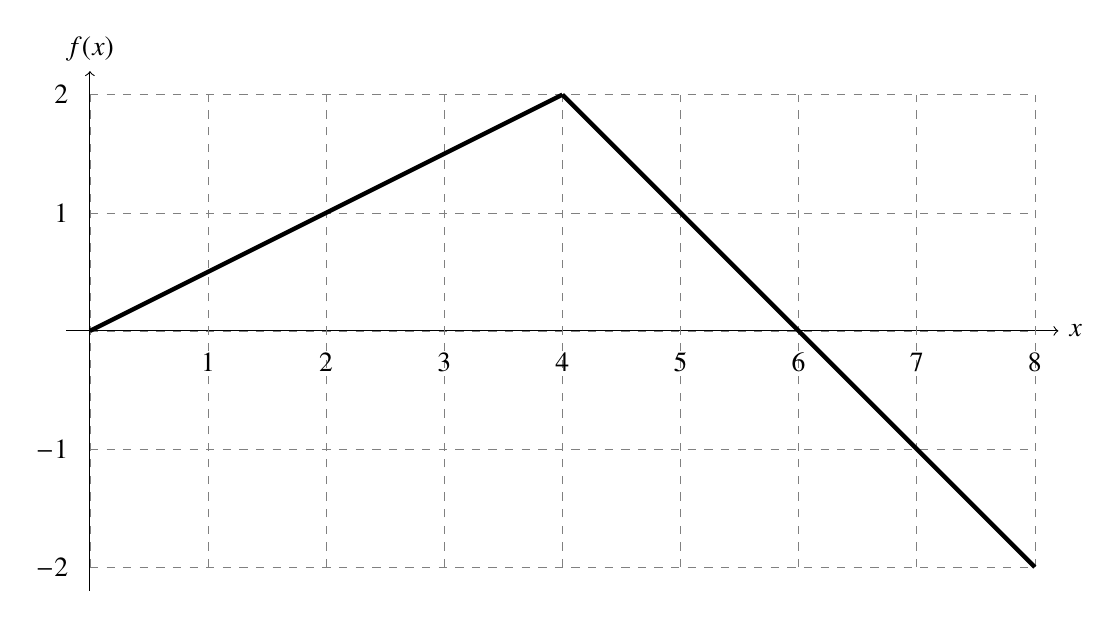
\begin{tikzpicture}[scale=1.5]
\draw[->] (-0.2,0) -- (8.2,0) node[right] {$x$};
\draw[->] (0,-2.2) -- (0,2.2) node[above] {$f(x)$};
\draw[help lines, dashed] (-0,-2) grid (8,2);
\draw[style= ultra thick] (0,0) --  (4,2) (4,2)--(8,-2);
%\draw[style= ultra thick] (0,1) arc (180:0:1);
\foreach \x in {1,2,...,8}
\draw (\x,-0.1) node[below] {$\x$};
\foreach \y in {-2,-1,1,2}
\draw (-0.1,\y) node[left] {$\y$};
\end{tikzpicture}
\end{center}

\bigskip
	\begin{enumerate}
\item What is the value of $f(4)$?

\vfill

\item  What is the value of $f'(2)$?

\vfill

\item  Evaluate $\ds \int_{2}^{7} f(x)\,dx$.

\vfill
\hspace*{-0.5in} The following questions concern $A(x) =\ds \int_0^x f(s)\,ds$. \\


\item  What is the value of $A(4)$?

\vfill

\item  What is the value of $A'(5)$.

\vfill

\item Does $A(x)$  have a maximum? Explain your answer.
\vfill
	\end{enumerate}

\newpage


\item (12 points) The temperature of a cup of coffee is modeled by the function $$f(t)=110e^{-t/10}+40$$ where $f$ is measured in degrees Fahrenheit and $t$ is measured in minutes after the coffee was poured into the cup.\\
	\begin{enumerate}
\item Compute $f'(0).$ Then explain what this number means in language the general public could understand.
\vfill
\item Compute $\ds \lim_{t \to \infty} f(t)$. Then explain what this number means in language the general public could understand.
\vfill
	\end{enumerate}

\newpage
%%%% related rate 
%%%% Drafted
\item (8 points) The radius of a spherical balloon is increasing at a rate of 2 cm/s. At what rate is the surface area of the balloon changing when the radius of the balloon is 5 cm? (Note that the surface area of a sphere is given by $SA=4\pi r^2.$) Include units with your answer.
\vspace{3in}
\end{enumerate}
%% Extra Credit Newton's Method
\textbf{Extra Credit} (5 points) The graph of the function $f(x)=\frac{1}{2}x^5-x-\frac{1}{4}\:$ is shown.

%\vskip -.7in

\begin{minipage}{0.5\textwidth}

	\subproblem{}
	Suppose Newton's method is used to find an approximate solution to
	$f(x)=0$ from an initial guess of $x_1=1$. Sketch on the graph how the
	next approximation $x_2$ will be found, labeling
	its location on the $x$-axis.
	\vskip 0.5 in
	\subproblem{} 
For $x_1=1$, give a formula for $x_2$. You do not need to
simplify, but your answer should be in a form where a calculator
would compute a numerical value.

\end{minipage}
\begin{minipage}{0.5\textwidth}

\hfill

	
	\begin{tikzpicture}[yscale=1.8,xscale=3.2]
\draw[->] (-0.5,0) -- (2.2,0) node[right] {$x$};
\draw[->] (0,-1.2) -- (0,2.2) node[above] {$f(x)$};
\draw[help lines, dashed] (-0,-1) grid (2,2);
\foreach \x in {1,2}
\draw (\x,-0.1) node[below] {$\x$};
\foreach \y in {1,2}
\draw (-0.1,\y) node[left] {$\y$};
%\draw[scale=0.5, domain=-3:3, smooth, variable=\x, blue] plot ({\x}, {\x*\x});
	\draw[domain=-0.5:1.5, -, ultra thick,smooth, variable=\x] plot({\x},{0.5*\x^5-\x-0.25});
	\end{tikzpicture}
\end{minipage}

\bigskip

\vfill

\vspace{1.0in}


\end{document}
